\documentclass[12pt,parskip=full]{article}
\usepackage{lmodern}
\usepackage{amsmath}
\usepackage[left=1.0in,right=1.0in,top=1.0in,bottom=1.0in]{geometry}
\geometry{letterpaper}
\usepackage{graphicx}
\usepackage{caption}
\usepackage{subcaption}
\usepackage{longtable}
\usepackage{float}
\usepackage{wrapfig}
\usepackage{soul}
\usepackage{textcomp}
\usepackage{marvosym}
\usepackage{wasysym}
\usepackage{latexsym}
\usepackage{amssymb}
\usepackage{apacite}
\usepackage{tabu}
\usepackage[svgnames]{xcolor}
\usepackage{tikz}
\usepackage[linktoc=all]{hyperref}
\usepackage{cleveref}
\usepackage{listings}
\usepackage{setspace}
\usepackage{parskip}
\usepackage{array}
\usepackage{apacite}
\usepackage{natbib}
\usepackage{multicol}
\usepackage{subcaption}
\usetikzlibrary{arrows}

\pgfdeclarelayer{edgelayer}
\pgfdeclarelayer{nodelayer}
\pgfsetlayers{edgelayer,nodelayer,main}

\tikzstyle{none}=[inner sep=0pt]
\tikzstyle{waypt}=[circle,fill=Black,draw=Black,scale=0.4]
\tikzstyle{Helobody}=[circle,fill=White,draw=Black,scale=4.0]
\tikzstyle{Tailrotor}=[circle,fill=White,draw=Black,scale=1.0]
\tikzstyle{ForceVector}=[->,draw=Indigo,fill=Indigo]
\tikzstyle{Coordinate}=[->,draw=Red,fill=Red,fill opacity=1.0]
\tikzstyle{angle}=[->]
\tikzstyle{MeasureMark}=[|-|]
\newlength{\imagewidth}
\newlength{\imagescale}

\setlength{\parskip}{11pt}
%\setlength{\parindent}{15pt}
\usepackage{bookmark}
\makeatletter
\renewcommand\@seccntformat[1]{}
\makeatother

\lstset
{
    language=Matlab,
    keywords={break,case,catch,continue,else,elseif,end,for,function,
        global,if,otherwise,persistent,return,switch,try,while},
    basicstyle=\ttfamily,
    keywordstyle=\color{blue},
    commentstyle=\color{ForestGreen},
    stringstyle=\color{purple},
    numbers=left,
    numberstyle=\tiny\color{gray},
    stepnumber=1,
    numbersep=10pt,
    backgroundcolor=\color{white},
    tabsize=4,
    showspaces=false,
    showstringspaces=false
}

\renewcommand{\thesection}{\arabic{section}}

\renewcommand{\thesubsection}{\thesection\alph{subsection}}
\renewcommand{\theequation}{\thesubsection\arabic{equation}}

\numberwithin{subsection}{section}

\begin{document}
	\vspace{-2ex}
	\title{Report 3: So Many Dimensions\vspace{-3.5ex}}
	\author{Rob Rau\vspace{-4ex}}
	\date{\today\vspace{-4ex}}
	\maketitle
	
	\section{What a Drag Part 2}
		Let's get straight to the point. The minimum drag value is $258.367 N$ with an aspect ratio of $14.2816$ and
		a reference planform area of $11.6682 m^2$. Now for the specifics. There's not much to say about the steepest
		descent optimizer. It behaved as expected, exhibiting the zig-zag pattern as it converged on the solution.
		The pattern would depend on the start point of course. Start points that were farther out would sometimes 
		head in a straight line as the gradient of successive points would be roughly in the same direction. This
		effect can be seen in \cref{fig:steepest}.
		
		\begin{figure}[!ht]
			\centering
			\begin{subfigure}[h]{0.3\textwidth}
				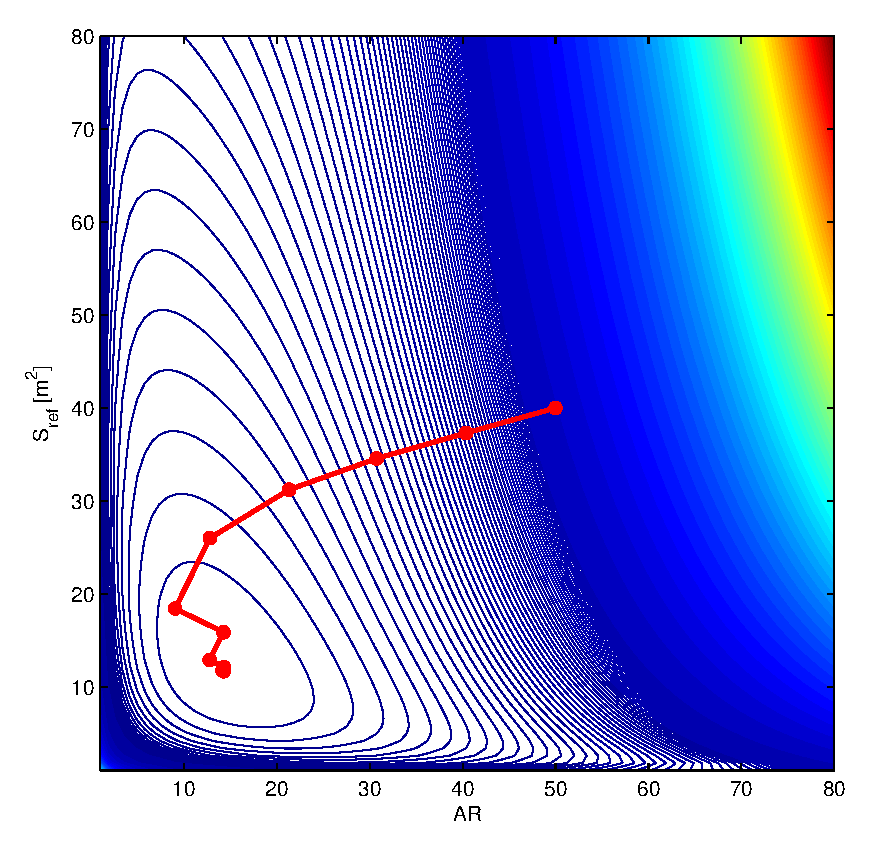
\includegraphics[width=\textwidth]{SteepestDrag1.eps}
				\subcaption{Drag minimization with start point of $AR = 50$, $S_{ref} = 40$}
			\end{subfigure}
			\begin{subfigure}[h]{0.3\textwidth}
				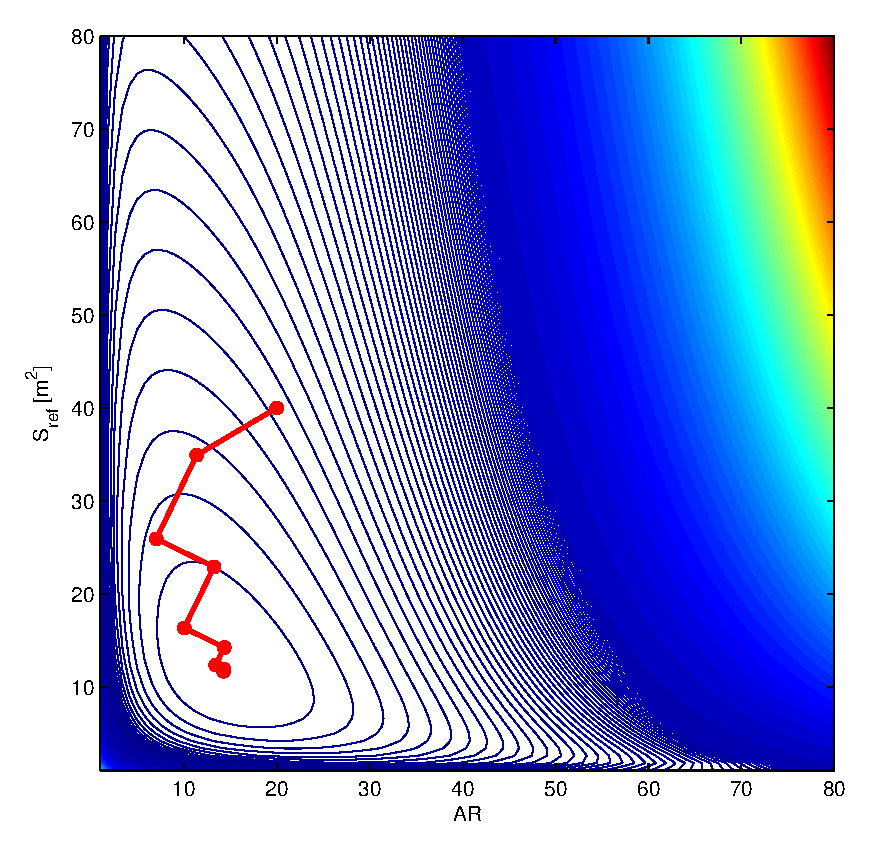
\includegraphics[width=\textwidth]{SteepestDrag2.eps}
				\subcaption{Drag minimization with start point of $AR = 20$, $S_{ref} = 40$}
			\end{subfigure}
			\begin{subfigure}[h]{0.3\textwidth}
				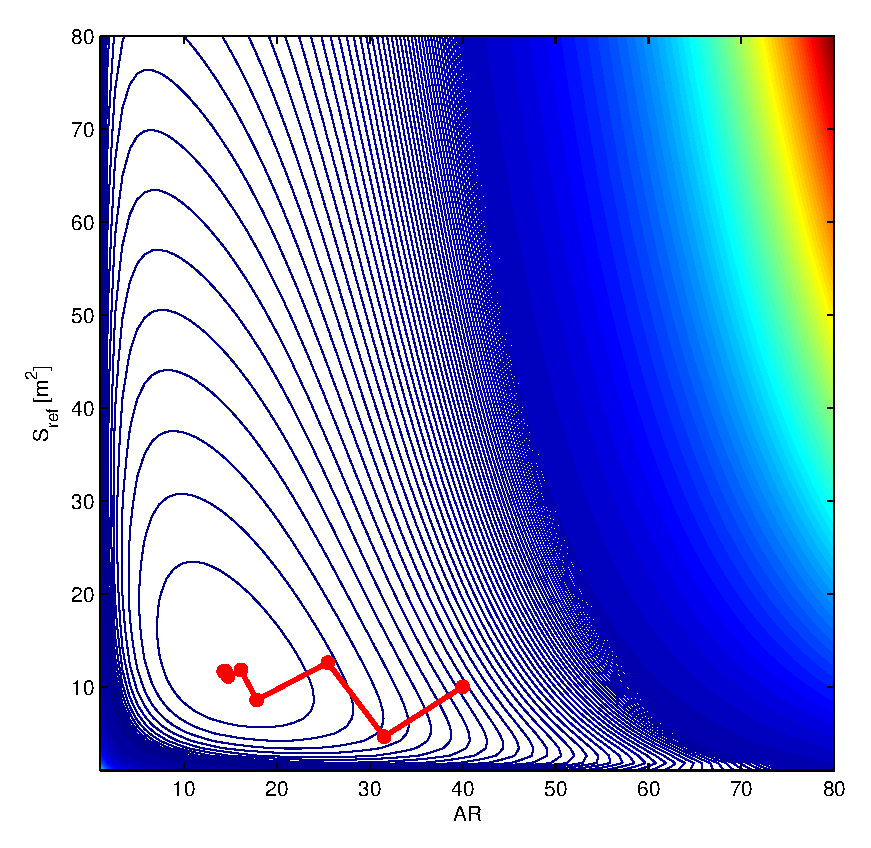
\includegraphics[width=\textwidth]{SteepestDrag3.eps}
				\subcaption{Drag minimization with start point of $AR = 40$, $S_{ref} = 10$}
			\end{subfigure}
			\caption{Comparison of start points for steepest descent method.\label{fig:steepest}}
		\end{figure}
		
		The conjugate gradient method I found to be a bit more interesting. I first coded up the conjugate gradient method
		using the Fletcher-Reeves update method. After some testing I wasn't particularly happy with this. It can be
		seen in \cref{tab:Drag1} through \cref{tab:Drag3} that the Fletcher-Reeves method wasn't performing much better
		than the steepest descent. I then decided to try the Polak-Ribi\`{e}re variant. I found that this method seemed
		to work better and more consistently that Fletcher-Reeves. I also did attempt the Dai-Yuan variant but could not
		get it to work at all. The paths of both methods can be seen in \cref{fig:conjGrad}
		\begin{figure}[!ht]
			\centering
			\begin{subfigure}[h]{0.4\textwidth}
				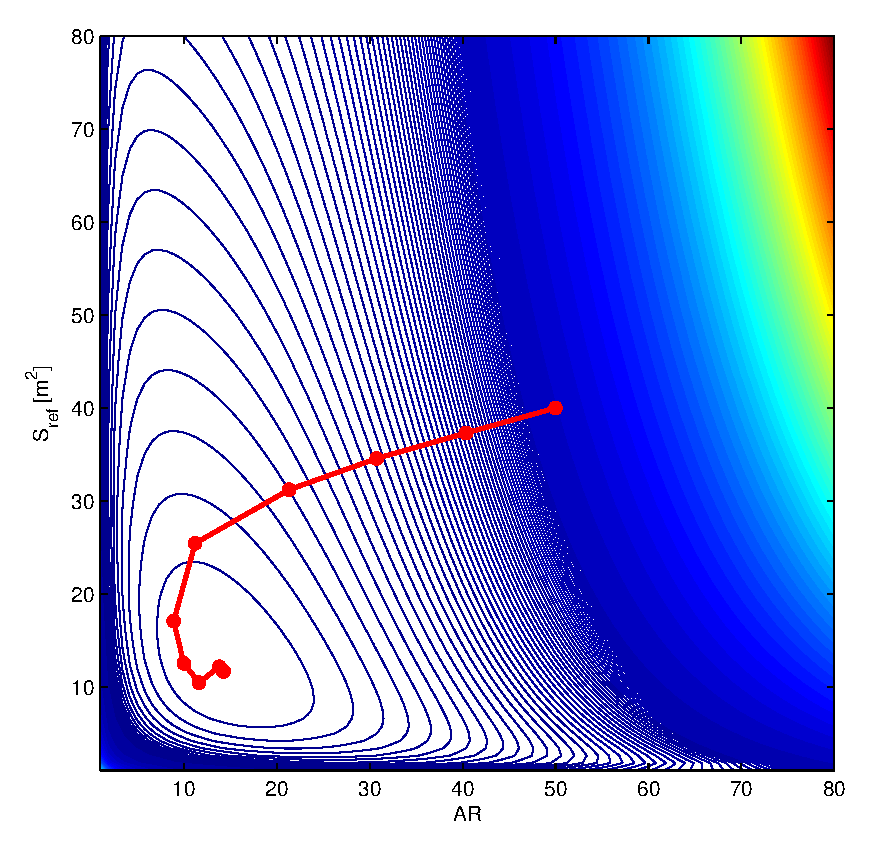
\includegraphics[width=\textwidth]{ConjGradFRDrag3.eps}
				\subcaption{Conjugate gradient using Fletcher-Reeves update with start point of $AR = 50$, $S_{ref} = 40$}
			\end{subfigure}
			\begin{subfigure}[h]{0.4\textwidth}
				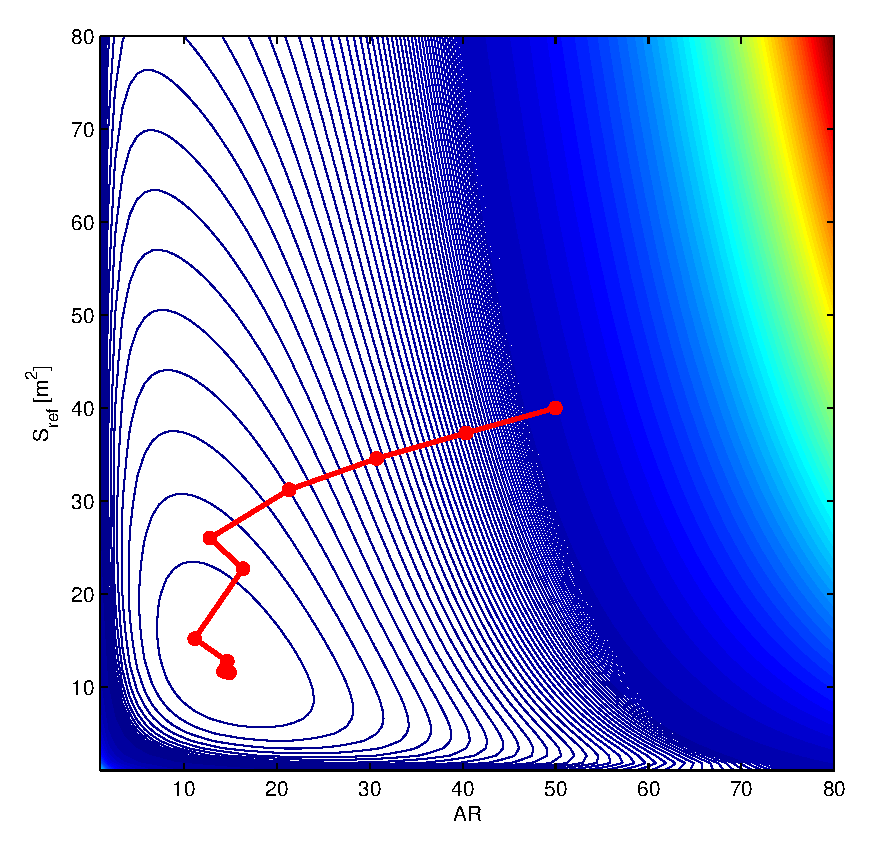
\includegraphics[width=\textwidth]{ConjGradPRDrag3.eps}
				\subcaption{Conjugate gradient using Polak-Ribi\`{e}re update with start point of $AR = 50$, $S_{ref} = 40$}
			\end{subfigure}
			\caption{Comparison of start points for steepest descent method.\label{fig:conjGrad}}
		\end{figure}
		
		For the quasi-newton method, I chose to use BFGS. While this method seemed like the most complex of the three (four)
		I coded, it actually turned out to be the easiest to debug. As expected BFGS converged much quicker than the other 
		methods discussed. As will be seen later, this method also performed the best with a large number of variables.
		The path this method took can be seen in \cref{fig:bfgsDrag}.
		
		\begin{center}
		    \captionof{table}{Drag minimization with start point of $AR = 50$, $S_{ref} = 40$} \label{tab:Drag1}
		    \begin{tabular}{ | l | c | c |}
		        \hline
		        Optimizer & Major Iterations & Minor Iterations \\ \noalign{\hrule height 2pt}
		        Steepest Descent & 13 & 273 \\ \hline
		        Conjugate Gradient (Fletcher-Reeves) & 14 & 292 \\ \hline
		        Conjugate Gradient (Polak-Ribi\`{e}re) & 12 & 282 \\ \hline
		        BFGS Quasi-Newton & 9 & 201 \\ \hline
		    \end{tabular}
		\end{center}
		
		\begin{center}
		    \captionof{table}{Drag minimization with start point of $AR = 20$, $S_{ref} = 40$} \label{tab:Drag2}
		    \begin{tabular}{ | l | c | c |}
		        \hline
		        Optimizer & Major Iterations & Minor Iterations \\ \noalign{\hrule height 2pt}
		        Steepest Descent & 11 & 229 \\ \hline
		        Conjugate Gradient (Fletcher-Reeves) & 11 & 234 \\ \hline
		        Conjugate Gradient (Polak-Ribi\`{e}re) & 8 & 173 \\ \hline
		        BFGS Quasi-Newton & 7 & 158 \\ \hline
		    \end{tabular}
		\end{center}
		
		\begin{center}
		    \captionof{table}{Drag minimization with start point of $AR = 40$, $S_{ref} = 10$} \label{tab:Drag3}
		    \begin{tabular}{ | l | c | c |}
		        \hline
		        Optimizer & Major Iterations & Minor Iterations \\ \noalign{\hrule height 2pt}
		        Steepest Descent & 11 & 230 \\ \hline
		        Conjugate Gradient (Fletcher-Reeves) & 9 & 191 \\ \hline
		        Conjugate Gradient (Polak-Ribi\`{e}re) & 10 & 212 \\ \hline
		        BFGS Quasi-Newton & 6 & 135 \\ \hline
		    \end{tabular}
		\end{center}
		
		
		\begin{figure}[!ht]
			\centering
			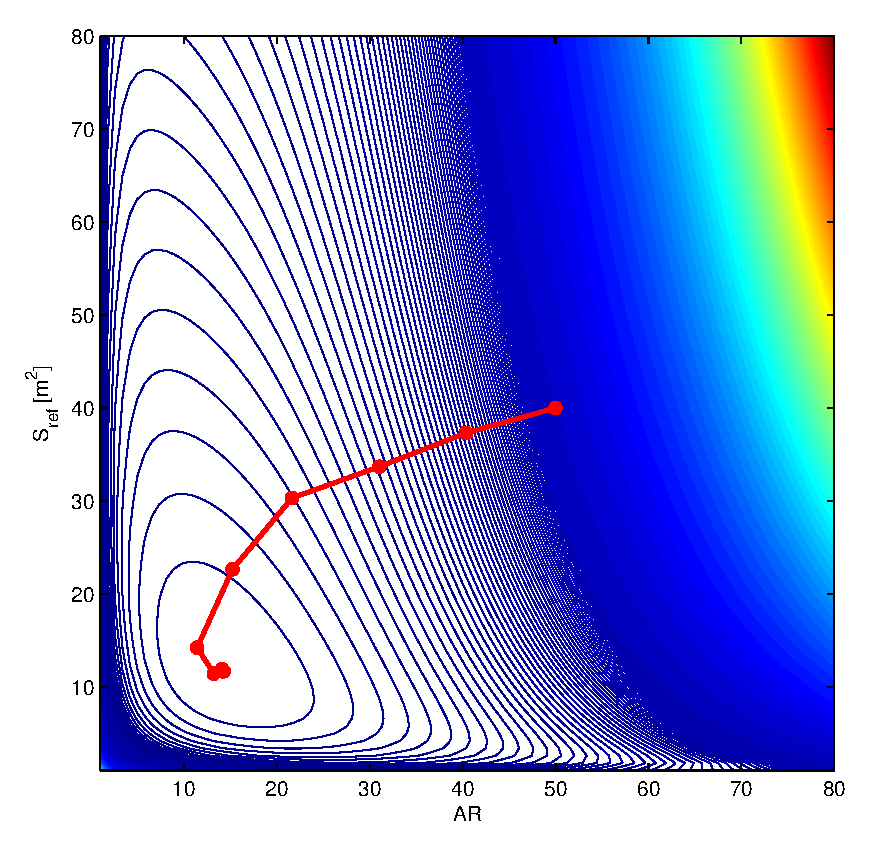
\includegraphics[scale=0.4]{BfgsDrag3.eps}
			\caption{BFGS drag minimization path with start point of $AR = 50$, $S_{ref} = 40$\label{fig:bfgsDrag}}
		\end{figure}
		
	\section{Convergence}
		The convergence of the various methods in the context of drag minimization can be seen in \cref{fig:dragConverg1}.
		The interesting thing here is the convergence of the Polak-Ribi\`{e}re method. All the other methods
		exhibit expected behavior, I currently have no explanation for this. To add to the mystery, the Polak-Ribi\`{e}re
		method seemed to perform better than the others.
		
		\begin{figure}[!ht]
			\centering
			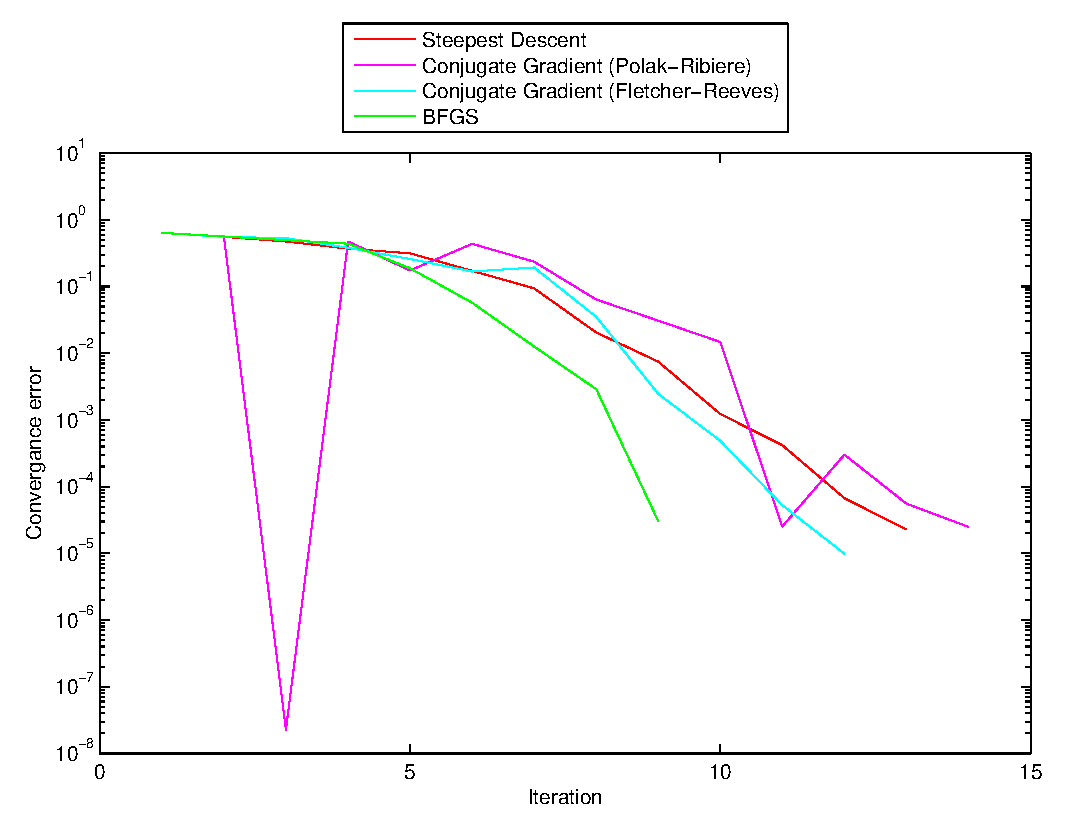
\includegraphics[scale=0.5]{DragConvergance.eps}
			\caption{Convergence of various methods with start point of $AR = 50$, $S_{ref} = 40$\label{fig:dragConverg1}}
		\end{figure}
	
		This may be an artifact of the specific problem. When looking at the convergence of the Rosenbrock function,
		the Polak-Ribi\`{e}re method behaves as expected. This can be seen in \cref{fig:Rose2DConverg}.
		
		\begin{figure}[!ht]
			\centering
			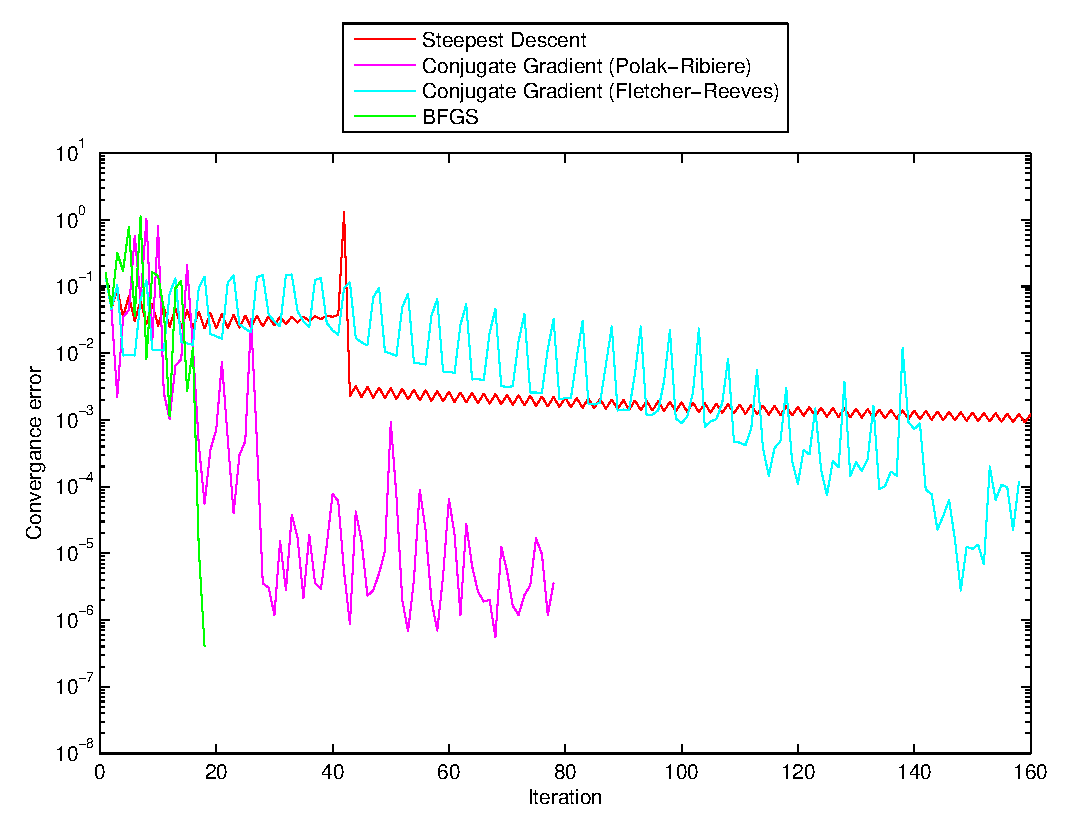
\includegraphics[scale=0.5]{Rose2DConvergance.eps}
			\caption{Convergence of various methods of the 2D Rosenbrock function\label{fig:Rose2DConverg}}
		\end{figure}
			
	\section{Effects of gradient precision}
		To test the effects of gradient precision, I decided to to switch my derivative method to finite
		differences as opposed to the complex step. I set the step size to something large ($1.0\times10^-2$)
		and let it go. On the drag minimization problem this didn't seem to have a huge effect. The results
		can be seen in \cref{tab:DragCD}.
		
		\begin{center}
		    \captionof{table}{Drag minimization using bad derivatives with start point of $AR = 50$, $S_{ref} = 40$} \label{tab:DragCD}
		    \begin{tabular}{ | l | c | c |}
		        \hline
		        Optimizer & Major Iterations & Minor Iterations \\ \noalign{\hrule height 2pt}
		        Steepest Descent & 13 & 273 \\ \hline
		        Conjugate Gradient (Fletcher-Reeves) & 12 & 260 \\ \hline
		        Conjugate Gradient (Polak-Ribi\`{e}re) & 12 & 260 \\ \hline
		        BFGS Quasi-Newton & 9 & 200 \\ \hline
		    \end{tabular}
		\end{center}
		
		To make things strange, the Fletcher-Reeves conjugate gradient method actually ended up performing better.
		
		As with the convergence, I found this effect to be more prominent and interesting when done to the
		Rosenbrock function.
		
		\begin{figure}[!ht]
			\centering
			\begin{subfigure}[h]{0.4\textwidth}
				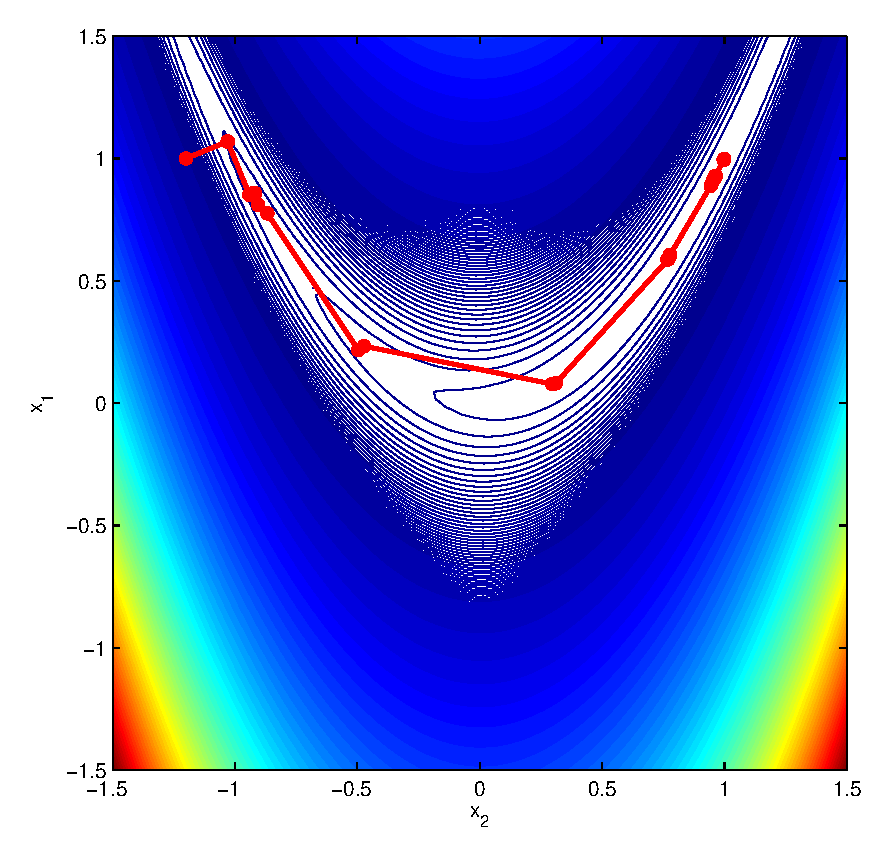
\includegraphics[width=\textwidth]{ConjGradPRRose.eps}
				\subcaption{Conjugate gradient using complex step derivatives. 53 major iterations}
			\end{subfigure}
			\begin{subfigure}[h]{0.4\textwidth}
				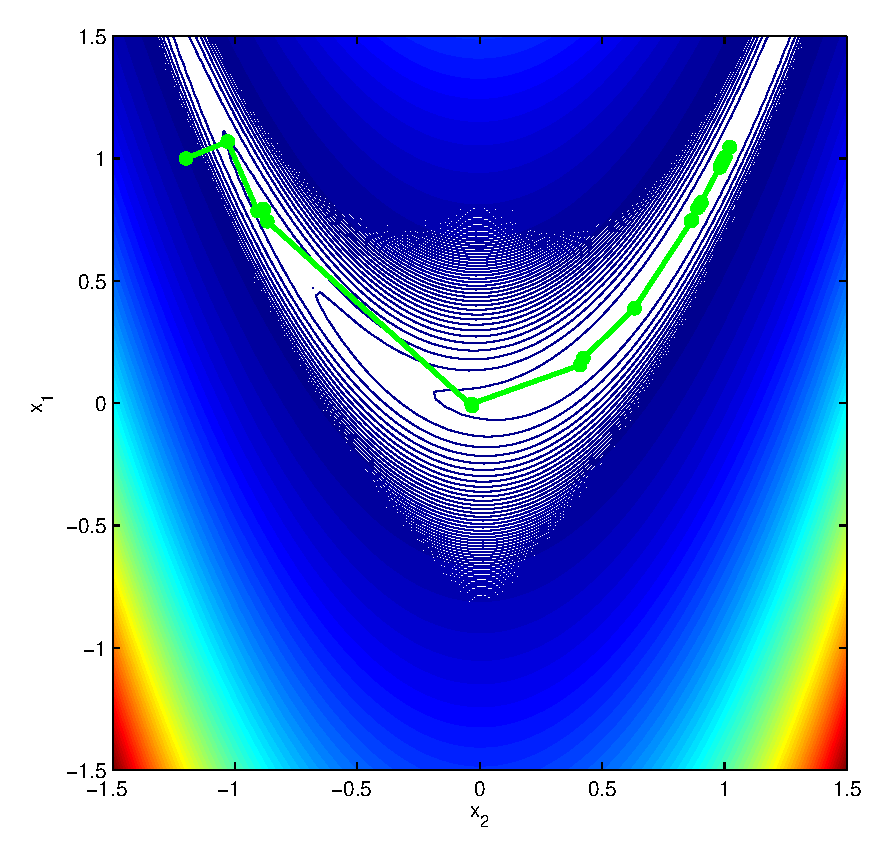
\includegraphics[width=\textwidth]{ConjGradPRRoseCD.eps}
				\subcaption{Conjugate gradient using finite difference derivatives. 15197 major iterations}
			\end{subfigure}
			\caption{Comparison of different derivative methods.\label{fig:RoseConjGradDer}}
		\end{figure}
	
		As \cref{fig:RoseConjGradDer} shows, the path taken by the optimizer is significantly different when
		using poor derivatives. It also took 3 orders of magnitude longer to converge!
		
		The precision of the derivatives also has an effect on the solution it finds. The optimal point of
		the Rosenbrock function is at (1.0, 1.0) with a value of 0. Using the complex step, BFGS
		would converge to a solution of (1.0, 0.99999999) with a function value of $4.3913\times 10^{-12}$.
		Using bad derivatives it converged to (0.981471, 0.963291) with a function value of 0.000343311.
		This is no good, we loose significant precision of our answer with this. This again is more prominent
		in the Rosenbrock function that it is with the drag function.
		
	\pagebreak
	\section{Rosenbrockly and the Effects of Dimensionality}
	
		Working on this problem is when I realized I wasn't happy with the Fletcher-Reeves conjugate gradient method
		and decided to try the Polak-Ribi\`{e}re method for updating $\beta$. As can be seen in \cref{fig:RoseConjGradComp}
		the Fletcher-Reeves conjugate gradient method seemed to take many small steps as it approaches the minimum.
		I played around with the parameters to try and improve it, but to no avail.
		\begin{figure}[!ht]
			\centering
			\begin{subfigure}[h]{0.4\textwidth}
				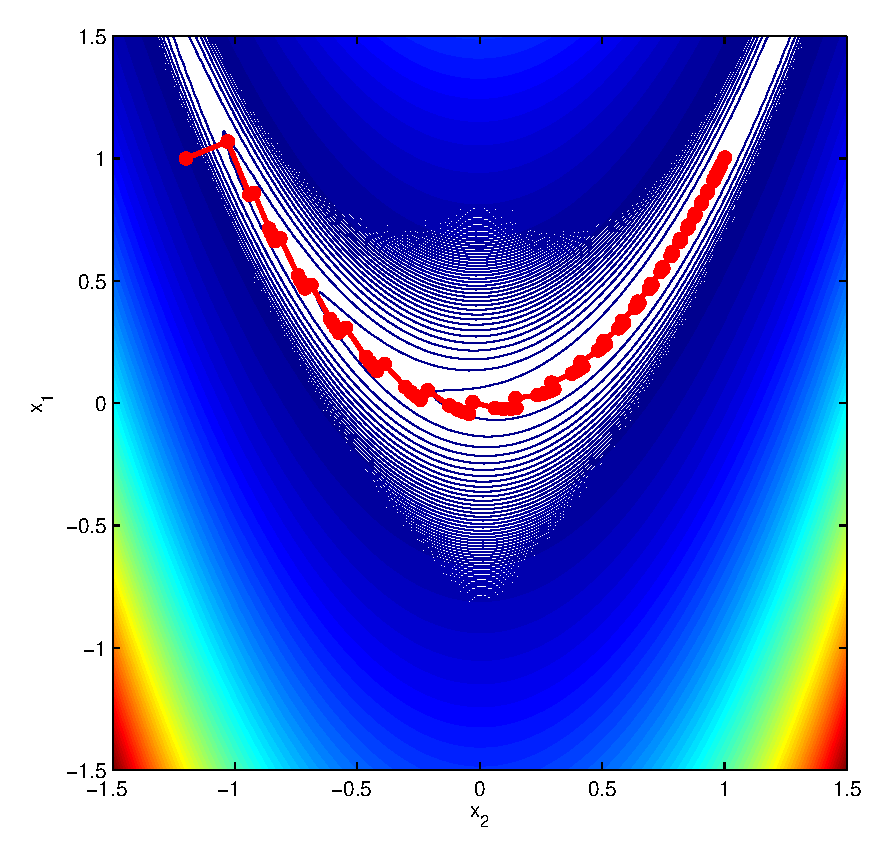
\includegraphics[width=\textwidth]{ConjGradFRRose.eps}
				\subcaption{Conjugate gradient using Fletcher-Reeves update.}
			\end{subfigure}
			\begin{subfigure}[h]{0.4\textwidth}
				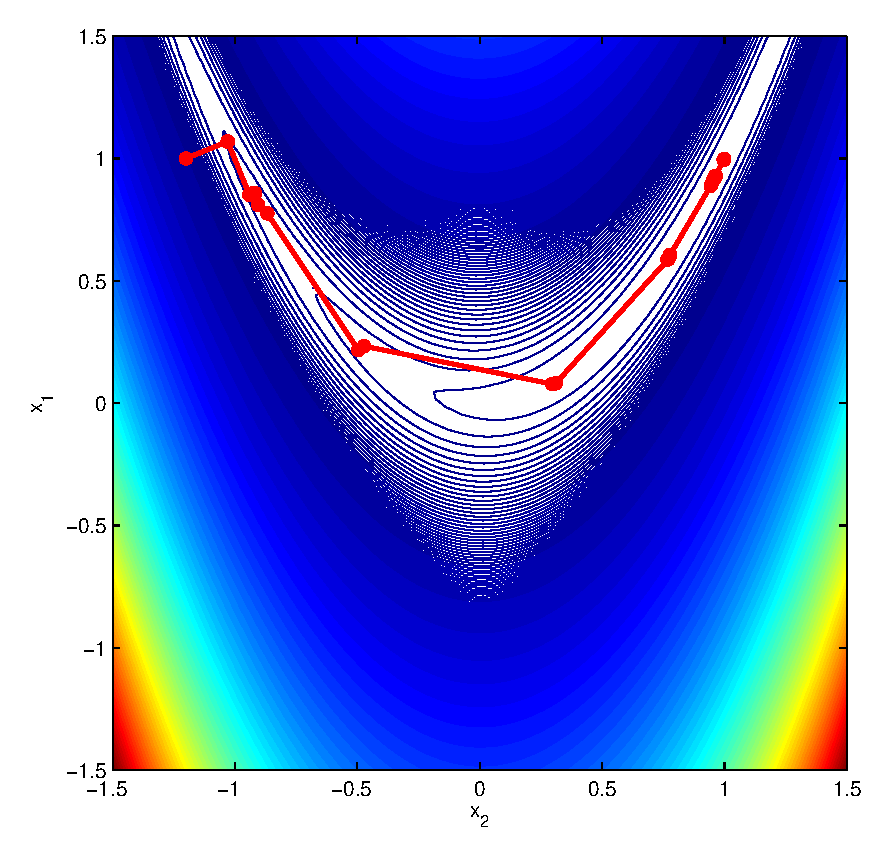
\includegraphics[width=\textwidth]{ConjGradPRRose.eps}
				\subcaption{Conjugate gradient using Polak-Ribi\`{e}re update.}
			\end{subfigure}
			\caption{Comparison of different conjugate gradient methods.\label{fig:RoseConjGradComp}}
		\end{figure}
		
		On the other hand, the Polak-Ribi\`{e}re method take a far more direct path to the minimum. Both
		these methods use the exact same line search with the same parameters. The only difference
		is how $\beta$ is updated. The other methods behaved as expected as seen in \cref{fig:RoseSteepBfgs}.

		\begin{figure}[!ht]
			\centering
			\begin{subfigure}[h]{0.4\textwidth}
				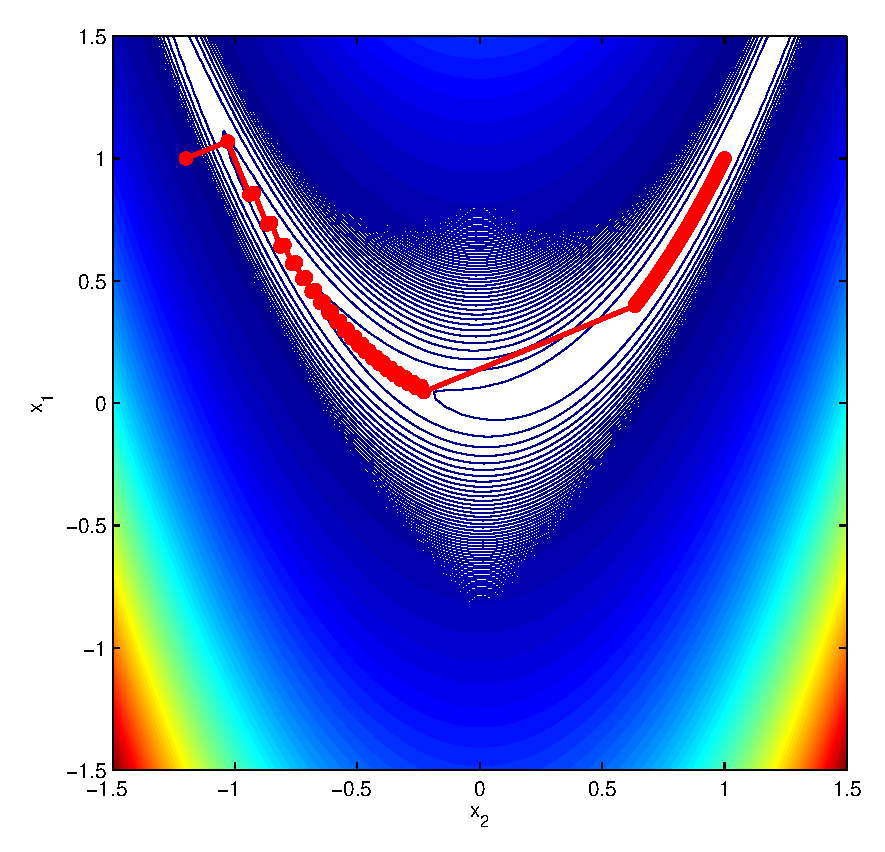
\includegraphics[width=\textwidth]{SteepestRose.eps}
				\subcaption{Steepest descent method on 2 dimensional Rosenbrock.}
			\end{subfigure}
			\begin{subfigure}[h]{0.4\textwidth}
				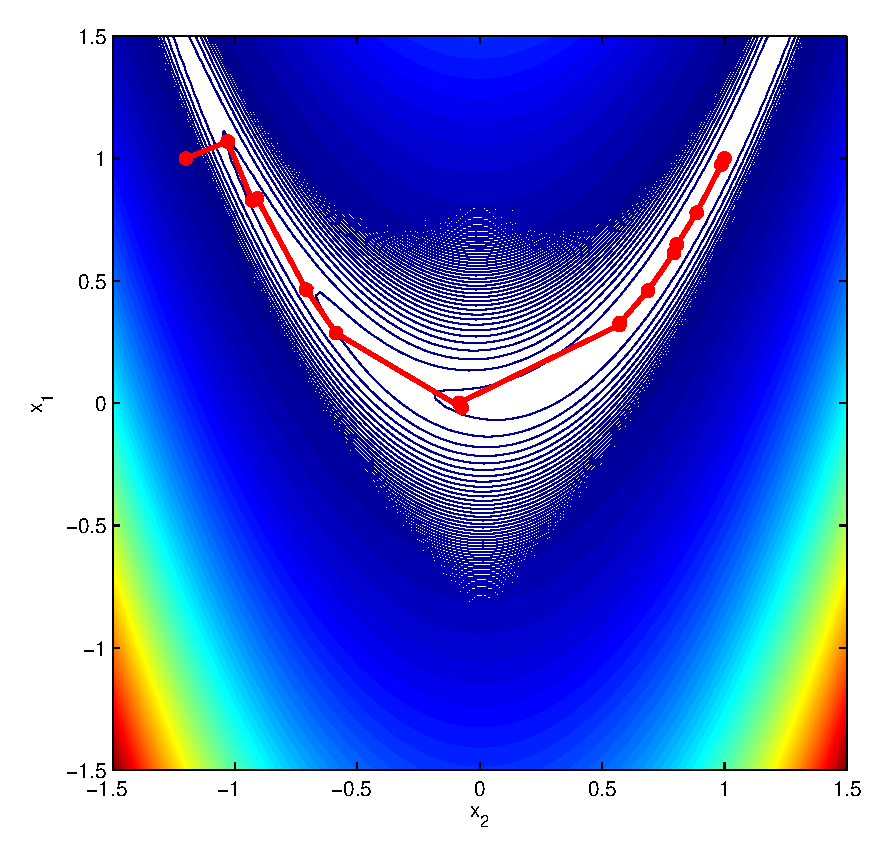
\includegraphics[width=\textwidth]{BfgsRose.eps}
				\subcaption{BFGS method on 2 dimensional Rosenbrock.}
			\end{subfigure}
			\caption{Steepest descent and BFGS on 2 dimensional Rosenbrock function.\label{fig:RoseSteepBfgs}}
		\end{figure}
		
		\subsection{Upping the Anti}
			So how does increasing the number of dimensions effect the number of iterations needed to find
			the minimum? This didn't turn out quite as I expected it to. The results can be seen in \cref{fig:IncDim}.
			
			\begin{figure}[!ht]
				\centering
				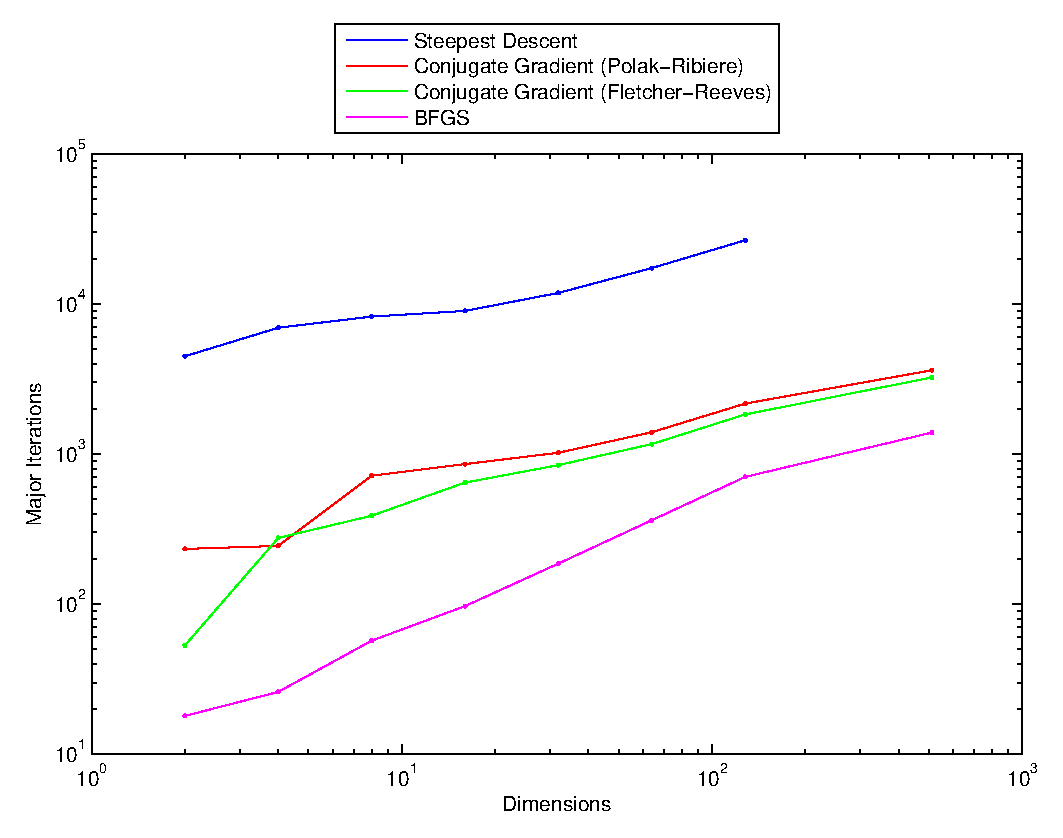
\includegraphics[scale=0.5]{DimensionEffect.eps}
				\caption{Number of major iterations required as number of dimensions increases.\label{fig:IncDim}}
			\end{figure}
			
			These results were more or less the opposite of what I expected. The steepest decent method, while
			still requires a large amount of iterations to converge, it seems to scale much better than the other
			methods. If this trend is consistent to higher dimensions, the steepest descent might actually 
			become the more efficient method. Unfortunately, due to time constraints, I was not able to test
			this to the extent that I wanted to. BFGS, while great for a low number of dimensions, does not 
			scale as well as even the conjugate gradient methods.
			
			This isn't the entire picture however. This analysis would be incomplete without looking at the
			effect on both the minor iterations and the total computation time. Interestingly \cref{fig:IncDimM}
			shows that the number of required minor iterations scales almost exactly as the major iterations.
			
			\begin{figure}[!ht]
				\centering
				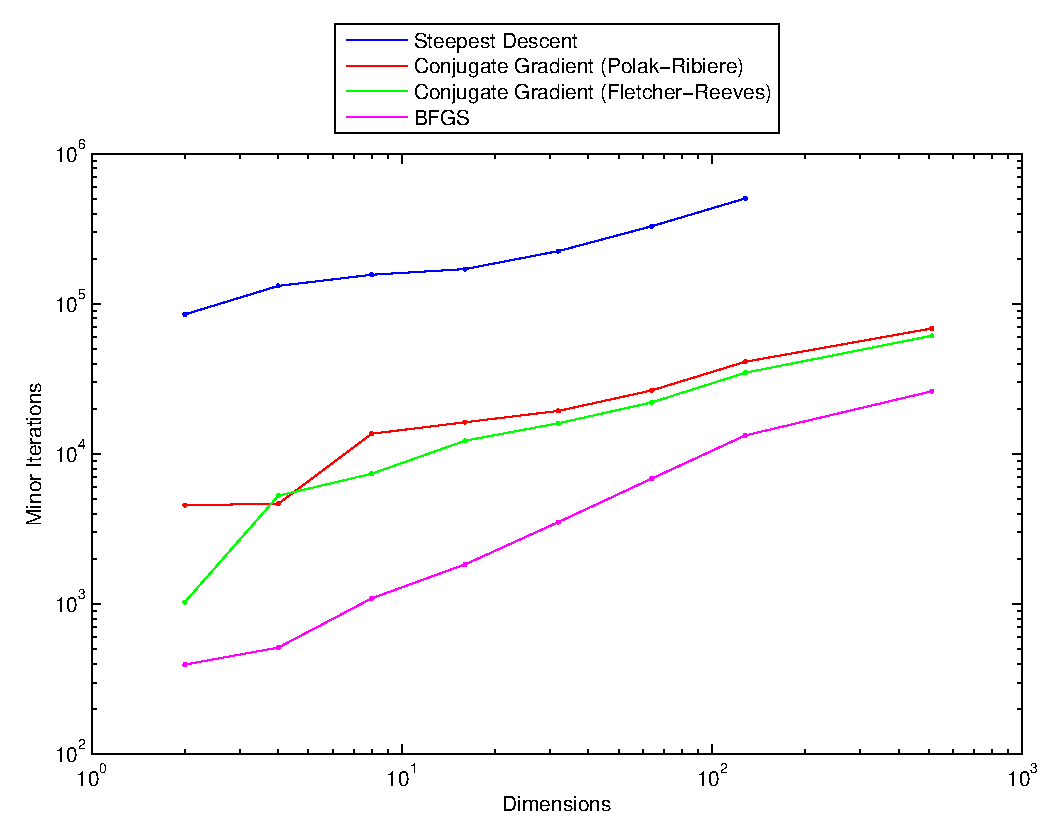
\includegraphics[scale=0.5]{DimensionEffectMinor.eps}
				\caption{Number of minor iterations required as number of dimensions increases.\label{fig:IncDimM}}
			\end{figure}
			
			But if we look at \cref{fig:IncDimT}, we see that in terms of total computation time, all methods
			scale very similarly.
			
			\begin{figure}[!ht]
				\centering
				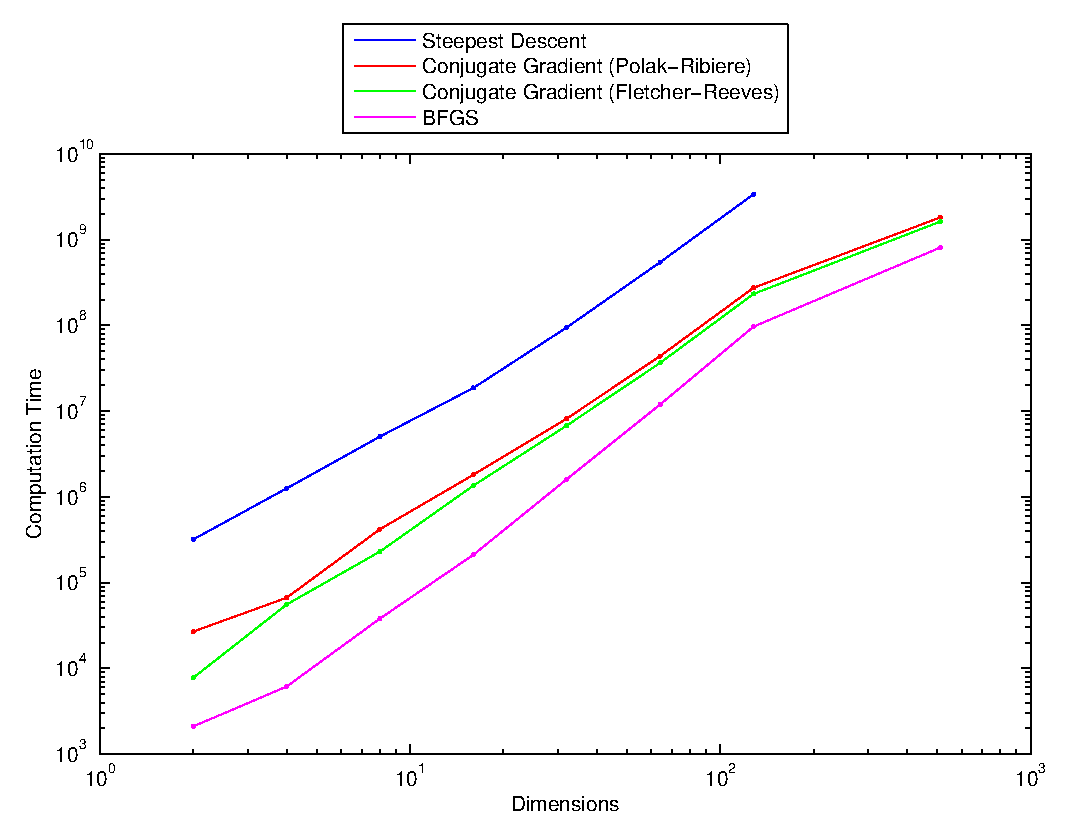
\includegraphics[scale=0.5]{DimensionEffectTime.eps}
				\caption{Total computation time as number of dimensions increases.\label{fig:IncDimT}}
			\end{figure}
			
			Unfortunately I did not have time to run the steepest descent for 512 dimensions.
			
			This will only run to 8 dimensions in the turned in version.
	
	\pagebreak
	\section{Performance}
		The BFGS quasi-newton method was far more effective than any of the other methods studied. As shown by
		the convergence, it performes very well, converging faster than anything else. Even when looking at
		the total computation time, BFGS scales just as well as any of the other methods.
		
		The conjugate gradient method ended up garnering most of time though. Comparing both the Fletcher-Reeves
		method and Polak-Ribi\`{e}re it's clear that the choice of how you pick $\beta$ has a significant impact
		on the effectiveness of the method.
		
		With both the conjugate gradient method and the BFGS method, there was a lot of tuning that can be done
		in regards to how frequently it resets either $\beta$ or the hessian update. This number seems to have
		a relatively large impact on the performance of the method.
		
		The steepest descent method is, of course, the slowest method. Its performance does however seem to
		depend largely on the problem. In well conditioned problem the steepest descent method could perform
		very well, but as we know, that is rarely the case.
\end{document}
